\chapter{Recurrent Neural Networks}
\label{chap:recurrent_networks}

\section*{Chapter Overview}

Recurrent Neural Networks (RNNs) process sequential data by maintaining hidden states that capture information from previous time steps. This chapter develops RNNs from basic recurrence to modern architectures like LSTMs and GRUs, establishing foundations for understanding transformers.

\subsection*{Learning Objectives}

\begin{enumerate}
    \item Understand recurrent architectures for sequential data
    \item Implement vanilla RNNs, LSTMs, and GRUs
    \item Understand vanishing/exploding gradient problems
    \item Apply RNNs to sequence modeling tasks
    \item Understand bidirectional and multi-layer RNNs
\end{enumerate}

\section{Vanilla RNNs}
\label{sec:vanilla_rnn}

\begin{definition}[Recurrent Neural Network]
\label{def:rnn}
An RNN processes sequence $\vx_1, \vx_2, \ldots, \vx_T$ by maintaining hidden state $\vh_t \in \R^h$:
\begin{align}
\vh_t &= \tanh(\mW_{hh} \vh_{t-1} + \mW_{xh} \vx_t + \vb_h) \\
\vy_t &= \mW_{hy} \vh_t + \vb_y
\end{align}
where:
\begin{itemize}
    \item $\mW_{hh} \in \R^{h \times h}$: hidden-to-hidden weights
    \item $\mW_{xh} \in \R^{h \times d}$: input-to-hidden weights
    \item $\mW_{hy} \in \R^{k \times h}$: hidden-to-output weights
    \item $\vh_0$ initialized (often zeros)
\end{itemize}
\end{definition}

\begin{figure}[h]
\centering
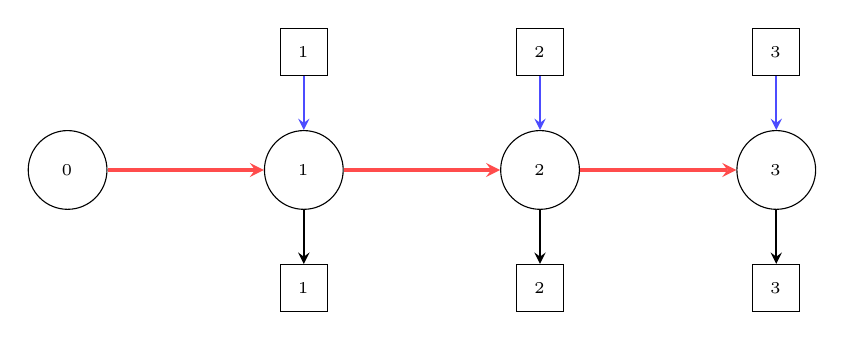
\begin{tikzpicture}[
    node/.style={circle, draw, minimum size=1cm, font=\small},
    input/.style={rectangle, draw, minimum size=0.6cm, font=\small},
    arrow/.style={->, >=stealth, thick},
    recurrent/.style={->, >=stealth, red!70, very thick}
]

% Hidden states
\node[node] (h0) at (0,0) {$\vh_0$};
\node[node] (h1) at (3,0) {$\vh_1$};
\node[node] (h2) at (6,0) {$\vh_2$};
\node[node] (h3) at (9,0) {$\vh_3$};

% Inputs
\node[input] (x1) at (3,1.5) {$\vx_1$};
\node[input] (x2) at (6,1.5) {$\vx_2$};
\node[input] (x3) at (9,1.5) {$\vx_3$};

% Outputs
\node[input] (y1) at (3,-1.5) {$\vy_1$};
\node[input] (y2) at (6,-1.5) {$\vy_2$};
\node[input] (y3) at (9,-1.5) {$\vy_3$};

% Recurrent connections (horizontal)
\draw[recurrent] (h0) -- (h1);
\draw[recurrent] (h1) -- (h2);
\draw[recurrent] (h2) -- (h3);

% Input connections (vertical)
\draw[arrow, blue!70] (x1) -- (h1);
\draw[arrow, blue!70] (x2) -- (h2);
\draw[arrow, blue!70] (x3) -- (h3);

% Output connections (vertical)
\draw[arrow] (h1) -- (y1);
\draw[arrow] (h2) -- (y2);
\draw[arrow] (h3) -- (y3);

\end{tikzpicture}
\caption{RNN unrolled through time showing sequential dependencies. Each hidden state $\vh_t$ depends on both the current input $\vx_t$ (blue arrows) and the previous hidden state $\vh_{t-1}$ (red arrows). The same weight matrices are shared across all time steps. This sequential structure prevents parallelization: $\vh_2$ cannot be computed until $\vh_1$ is complete.}
\label{fig:rnn_unrolled}
\end{figure}

\begin{example}[RNN Forward Pass]
\label{ex:rnn_forward}
Character-level language model with vocabulary size $V=5$, hidden size $h=3$.

Input sequence: "hello" encoded as one-hot vectors $\vx_1, \ldots, \vx_5 \in \R^5$

Initialize: $\vh_0 = [0, 0, 0]\transpose$

\textbf{Time step 1:} Process 'h'
\begin{align}
\vh_1 &= \tanh(\mW_{hh}\vh_0 + \mW_{xh}\vx_1 + \vb_h) \in \R^3 \\
\vy_1 &= \mW_{hy}\vh_1 + \vb_y \in \R^5 \\
\hat{\mathbf{p}}_1 &= \text{softmax}(\vy_1) \quad \text{(predict next character)}
\end{align}

\textbf{Time step 2:} Process 'e' using $\vh_1$
\begin{equation}
\vh_2 = \tanh(\mW_{hh}\vh_1 + \mW_{xh}\vx_2 + \vb_h)
\end{equation}

Hidden state $\vh_t$ carries information from all previous time steps.
\end{example}

\subsection{Backpropagation Through Time (BPTT)}

\begin{algorithm}[H]
\caption{Backpropagation Through Time}
\label{alg:bptt}
\KwIn{Sequence $\{\vx_1, \ldots, \vx_T\}$, targets $\{\vy_1, \ldots, \vy_T\}$}
\KwOut{Gradients for all parameters}

\tcp{Forward Pass}
\For{$t = 1$ \KwTo $T$}{
    $\vh_t = \tanh(\mW_{hh}\vh_{t-1} + \mW_{xh}\vx_t + \vb_h)$ \\
    $\vy_t = \mW_{hy}\vh_t + \vb_y$ \\
    $L_t = \text{Loss}(\vy_t, \text{target}_t)$
}

\tcp{Backward Pass}
Initialize $\frac{\partial L}{\partial \vh_{T+1}} = \mathbf{0}$ \\
\For{$t = T$ \KwTo $1$}{
    Compute $\frac{\partial L}{\partial \vh_t}$ (includes gradient from $t+1$) \\
    Accumulate $\frac{\partial L}{\partial \mW_{hh}}, \frac{\partial L}{\partial \mW_{xh}}, \frac{\partial L}{\partial \mW_{hy}}$
}
\end{algorithm}

\subsection{Vanishing and Exploding Gradients}

The fundamental challenge in training RNNs on long sequences arises from the multiplicative nature of gradient backpropagation through time. When computing gradients with respect to early hidden states, the chain rule requires multiplying Jacobian matrices across all intermediate time steps, leading to exponential growth or decay of gradient magnitudes.

The gradient of the loss with respect to an early hidden state $\vh_0$ involves the product of Jacobians across all time steps:
\begin{equation}
\frac{\partial \vh_T}{\partial \vh_0} = \prod_{t=1}^{T} \frac{\partial \vh_t}{\partial \vh_{t-1}} = \prod_{t=1}^{T} \mW_{hh}\transpose \text{diag}(\tanh'(\vz_t))
\end{equation}
where $\vz_t$ is the pre-activation at time $t$. Each Jacobian $\frac{\partial \vh_t}{\partial \vh_{t-1}}$ has spectral norm bounded by $\norm{\mW_{hh}} \cdot \norm{\text{diag}(\tanh'(\vz_t))}$. Since $\tanh'(z) \in (0, 1]$ with maximum value 1 at $z = 0$, the derivative term is at most 1 and typically much smaller for saturated activations. This means the Jacobian norm is approximately $\norm{\mW_{hh}}$ in the best case.

For a sequence of length $T = 100$, if $\norm{\mW_{hh}} = 0.95$ (slightly less than 1), the gradient magnitude decays as $0.95^{100} \approx 0.006$, reducing gradients by a factor of 167. If $\norm{\mW_{hh}} = 0.9$, the decay is $0.9^{100} \approx 2.7 \times 10^{-5}$, reducing gradients by a factor of 37,000. This exponential decay makes it nearly impossible for the network to learn long-range dependencies: the gradient signal from time step 100 is effectively zero by the time it reaches time step 0. In practice, vanilla RNNs struggle to learn dependencies longer than 10-20 time steps due to vanishing gradients.

Conversely, if $\norm{\mW_{hh}} = 1.05$, the gradient magnitude grows as $1.05^{100} \approx 131.5$, amplifying gradients by a factor of 131. If $\norm{\mW_{hh}} = 1.1$, the growth is $1.1^{100} \approx 13{,}781$, causing gradients to explode. Exploding gradients lead to numerical overflow (NaN values) and training instability, where loss suddenly spikes to infinity. While gradient clipping (capping gradient norms at a threshold like 1.0) provides a practical solution for exploding gradients, it does not address the fundamental problem of vanishing gradients.

The vanishing gradient problem is particularly severe because the spectral norm of $\mW_{hh}$ must be precisely 1.0 to avoid both vanishing and exploding gradients, and maintaining this property during training is extremely difficult. Initialization schemes like orthogonal initialization set $\mW_{hh}$ to have spectral norm 1.0 initially, but gradient descent updates quickly perturb this property. Even with careful initialization, vanilla RNNs rarely learn dependencies beyond 20-30 time steps in practice.

\subsection{Quantitative Analysis of Gradient Decay}

To understand the severity of vanishing gradients, consider a concrete example with BERT-base dimensions. Suppose we have a vanilla RNN with hidden dimension $h = 768$ (matching BERT-base) and sequence length $n = 512$ (BERT's maximum sequence length). The recurrence matrix $\mW_{hh} \in \R^{768 \times 768}$ has 589,824 parameters. If we initialize $\mW_{hh}$ orthogonally (spectral norm exactly 1.0) and the $\tanh$ derivatives average 0.5 (typical for non-saturated activations), the effective Jacobian norm per time step is approximately $1.0 \times 0.5 = 0.5$.

Over 512 time steps, the gradient magnitude decays as $0.5^{512} \approx 10^{-154}$, which is far below machine precision for FP32 (approximately $10^{-38}$) or even FP64 (approximately $10^{-308}$). The gradient effectively becomes exactly zero after about 130 time steps in FP32 or 1,000 time steps in FP64. This means a vanilla RNN cannot learn any dependencies spanning more than 130 tokens when using FP32 arithmetic, regardless of optimization algorithm or learning rate. The mathematical structure of the recurrence fundamentally limits the learnable dependency length.

For comparison, consider the gradient flow in a transformer with the same dimensions. The self-attention mechanism computes attention scores $\mA = \text{softmax}(\frac{\mQ\mK\transpose}{\sqrt{d_k}})$ and outputs $\mO = \mA\mV$. The gradient $\frac{\partial L}{\partial \mV}$ flows directly from the output through the attention weights, without any multiplicative accumulation across time steps. The gradient magnitude remains approximately constant regardless of sequence length, enabling transformers to learn dependencies spanning thousands of tokens. This fundamental difference in gradient flow explains why transformers replaced RNNs for nearly all sequence modeling tasks: they solve the vanishing gradient problem by design.

The LSTM architecture addresses vanishing gradients through its cell state mechanism, which provides an additive path for gradient flow. The cell state update $\mathbf{c}_t = \vf_t \odot \mathbf{c}_{t-1} + \vi_t \odot \tilde{\mathbf{c}}_t$ includes an additive term rather than purely multiplicative updates. The gradient with respect to $\mathbf{c}_{t-1}$ is:
\begin{equation}
\frac{\partial \mathbf{c}_t}{\partial \mathbf{c}_{t-1}} = \text{diag}(\vf_t)
\end{equation}
which is a diagonal matrix with entries in $(0, 1)$ determined by the forget gate. If the forget gate learns to output values close to 1 for important information, the gradient can flow backward through many time steps without vanishing. However, this requires the network to learn appropriate forget gate values, and in practice, LSTMs still struggle with dependencies beyond 100-200 time steps. The cell state provides a highway for gradients, but it does not eliminate the vanishing gradient problem entirely.

\section{Long Short-Term Memory (LSTM)}
\label{sec:lstm}

\begin{definition}[LSTM Cell]
\label{def:lstm}
LSTM uses gating mechanisms to control information flow:
\begin{align}
\vf_t &= \sigma(\mW_f[\vh_{t-1}, \vx_t] + \vb_f) && \text{(forget gate)} \\
\vi_t &= \sigma(\mW_i[\vh_{t-1}, \vx_t] + \vb_i) && \text{(input gate)} \\
\tilde{\mathbf{c}}_t &= \tanh(\mW_c[\vh_{t-1}, \vx_t] + \vb_c) && \text{(candidate cell)} \\
\mathbf{c}_t &= \vf_t \odot \mathbf{c}_{t-1} + \vi_t \odot \tilde{\mathbf{c}}_t && \text{(cell state)} \\
\vo_t &= \sigma(\mW_o[\vh_{t-1}, \vx_t] + \vb_o) && \text{(output gate)} \\
\vh_t &= \vo_t \odot \tanh(\mathbf{c}_t) && \text{(hidden state)}
\end{align}
where $\sigma$ is sigmoid, $\odot$ is element-wise multiplication, and $[\cdot, \cdot]$ is concatenation.
\end{definition}

\textbf{Key components:}
\begin{itemize}
    \item \textbf{Cell state $\mathbf{c}_t$:} Long-term memory, flows with minimal modification
    \item \textbf{Forget gate $\vf_t$:} What to remove from cell state
    \item \textbf{Input gate $\vi_t$:} What new information to store
    \item \textbf{Output gate $\vo_t$:} What to output from cell state
\end{itemize}

\begin{figure}[h]
\centering
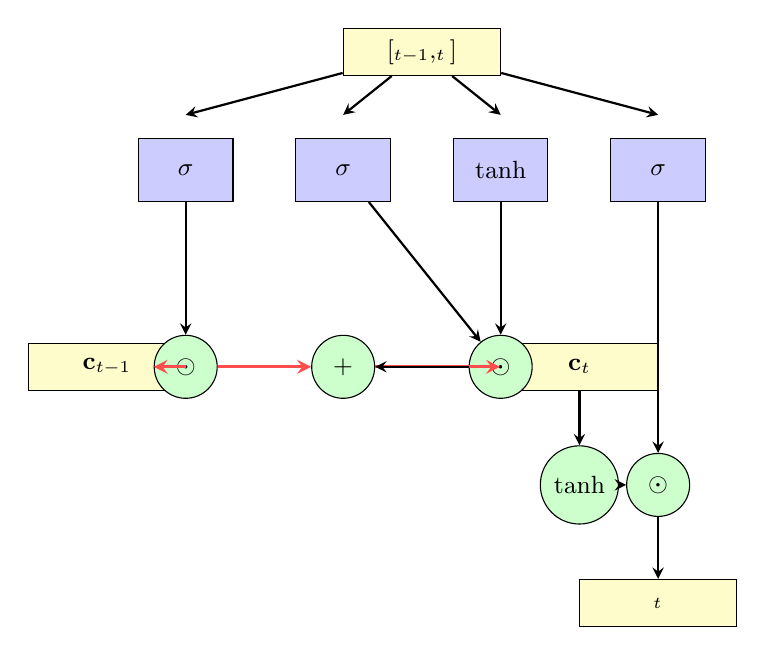
\begin{tikzpicture}[
    gate/.style={rectangle, draw, fill=blue!20, minimum width=1.2cm, minimum height=0.8cm, font=\small},
    operation/.style={circle, draw, fill=green!20, minimum size=0.8cm, font=\small},
    state/.style={rectangle, draw, fill=yellow!20, minimum width=2cm, minimum height=0.6cm, font=\small},
    arrow/.style={->, >=stealth, thick},
    cell_flow/.style={->, >=stealth, very thick, red!70}
]

% Inputs at top
\node[state] (input) at (0,4) {$[\vh_{t-1}, \vx_t]$};

% Four gates
\node[gate] (forget) at (-3,2.5) {$\sigma$};
\node[gate] (input_gate) at (-1,2.5) {$\sigma$};
\node[gate] (candidate) at (1,2.5) {$\tanh$};
\node[gate] (output_gate) at (3,2.5) {$\sigma$};

% Cell state flow (horizontal)
\node[state] (c_prev) at (-4,0) {$\mathbf{c}_{t-1}$};
\node[state] (c_curr) at (2,0) {$\mathbf{c}_t$};

% Operations
\node[operation] (mult1) at (-3,0) {$\odot$};
\node[operation] (mult2) at (1,0) {$\odot$};
\node[operation] (add) at (-1,0) {$+$};
\node[operation] (tanh_c) at (2,-1.5) {$\tanh$};
\node[operation] (mult3) at (3,-1.5) {$\odot$};

% Hidden state output
\node[state] (h_out) at (3,-3) {$\vh_t$};

% Connections from input to gates
\draw[arrow] (input) -- (-3,3.2);
\draw[arrow] (input) -- (-1,3.2);
\draw[arrow] (input) -- (1,3.2);
\draw[arrow] (input) -- (3,3.2);

% Gate outputs to operations
\draw[arrow] (forget) -- (mult1);
\draw[arrow] (input_gate) -- (mult2);
\draw[arrow] (candidate) -- (mult2);
\draw[arrow] (output_gate) -- (mult3);

% Cell state flow (the "highway")
\draw[cell_flow] (c_prev) -- (mult1);
\draw[cell_flow] (mult1) -- (add);
\draw[cell_flow] (add) -- (c_curr);
\draw[arrow] (mult2) -- (add);

% Cell to output
\draw[arrow] (c_curr) -- (tanh_c);
\draw[arrow] (tanh_c) -- (mult3);
\draw[arrow] (mult3) -- (h_out);

\end{tikzpicture}
\caption{LSTM cell internal structure showing the four gates and cell state flow. The cell state $\mathbf{c}_t$ (red path) provides an additive "highway" for gradient flow, addressing the vanishing gradient problem. The forget gate $\vf_t$ controls what to keep from $\mathbf{c}_{t-1}$, the input gate $\vi_t$ and candidate $\tilde{\mathbf{c}}_t$ control what new information to add, and the output gate $\vo_t$ controls what to output. All gates receive the same input $[\vh_{t-1}, \vx_t]$ but learn different transformations.}
\label{fig:lstm_gates}
\end{figure}

\begin{example}[LSTM Parameter Count]
\label{ex:lstm_params}
For input dimension $d=512$ and hidden dimension $h=1024$:

Each gate has weight matrix for $[\vh_{t-1}, \vx_t] \in \R^{h+d}$:
\begin{align}
\text{Single gate:} \quad &(h+d) \times h + h = (1024 + 512) \times 1024 + 1024 \\
&= 1{,}572{,}864 + 1{,}024 = 1{,}573{,}888
\end{align}

LSTM has 4 gates (forget, input, cell, output):
\begin{equation}
\text{Total:} \quad 4 \times 1{,}573{,}888 = 6{,}295{,}552 \text{ parameters}
\end{equation}

Compare to transformer attention with same dimensions: often fewer parameters and better parallelization!
\end{example}

\subsection{LSTM Computational Analysis}

Understanding the computational cost of LSTMs is essential for comparing them to transformers and explaining why transformers have become dominant despite LSTMs' theoretical advantages for sequential processing. The LSTM's gating mechanisms provide powerful modeling capabilities but come with significant computational overhead that limits their efficiency on modern hardware.

For an LSTM with input dimension $d$ and hidden dimension $h$, each time step requires computing four gates (forget, input, candidate, output), each involving a matrix multiplication with the concatenated input $[\vh_{t-1}, \vx_t] \in \R^{h+d}$. The computational cost per time step is:
\begin{equation}
\text{FLOPs per step} = 4 \times 2h(h+d) = 8h(h+d)
\end{equation}
where the factor of 2 accounts for multiply-accumulate operations, and the factor of 4 accounts for the four gates. For BERT-base dimensions with $d = h = 768$, this gives $8 \times 768 \times (768 + 768) = 9{,}437{,}184$ FLOPs per time step. For a sequence of length $n = 512$, the total cost is $512 \times 9{,}437{,}184 = 4{,}831{,}838{,}208$ FLOPs, or approximately 4.8 GFLOPs.

This computational cost is deceptively modest compared to transformers. A single transformer layer with the same dimensions requires approximately 12.9 GFLOPs for self-attention (with $n = 512$) plus 9.4 GFLOPs for the feed-forward network, totaling 22.3 GFLOPs—about 4.6× more than the LSTM. However, this comparison is misleading because it ignores the critical difference in parallelization: the transformer can process all 512 positions simultaneously, while the LSTM must process them sequentially.

The sequential nature of LSTMs means that the 4.8 GFLOPs cannot be parallelized across time steps. On an NVIDIA A100 GPU with peak throughput of 312 TFLOPS (FP16), the theoretical minimum time to process a sequence of length 512 is $\frac{4.8 \times 10^9}{312 \times 10^{12}} = 15.4$ microseconds if we could achieve perfect parallelization. However, the sequential dependency forces us to process one time step at a time, with each step taking approximately $\frac{9.4 \times 10^6}{312 \times 10^{12}} = 0.03$ microseconds at peak throughput. In practice, small matrix multiplications achieve only 1-5\% of peak throughput due to insufficient parallelism, so each time step actually takes approximately 1-3 microseconds, giving a total sequence processing time of 512-1,536 microseconds (0.5-1.5 milliseconds).

For comparison, a transformer layer can process the entire sequence in parallel. The self-attention computation requires three matrix multiplications ($\mQ = \mX\mW_Q$, $\mK = \mX\mW_K$, $\mV = \mX\mW_V$) with dimensions $512 \times 768 \times 768$, followed by the attention score computation $\mA = \text{softmax}(\frac{\mQ\mK\transpose}{\sqrt{d_k}})$ and output computation $\mO = \mA\mV$. These operations can be batched into large matrix multiplications that achieve 40-60\% of peak GPU throughput, completing in approximately 50-100 microseconds total. The transformer is 5-30× faster than the LSTM despite having more FLOPs, purely due to better parallelization.

The memory requirements for LSTM hidden states are modest compared to transformer attention matrices. For batch size $B$ and sequence length $n$, the LSTM must store hidden states $\vh_t \in \R^{B \times h}$ and cell states $\mathbf{c}_t \in \R^{B \times h}$ for each time step, requiring $2Bnh \times 4 = 8Bnh$ bytes in FP32. For BERT-base dimensions with $B = 32$, $n = 512$, $h = 768$, this totals $8 \times 32 \times 512 \times 768 = 100{,}663{,}296$ bytes, or approximately 96 MB. This is substantially less than the 384 MB required for transformer attention scores in a single layer, making LSTMs more memory-efficient for long sequences.

However, this memory advantage is offset by the sequential processing requirement. While transformers can trade memory for speed by using gradient checkpointing (recomputing activations during the backward pass rather than storing them), LSTMs cannot benefit from this technique as effectively because the sequential dependency prevents parallelization of the recomputation. Gradient checkpointing reduces transformer memory by 3-5× with only 20-30\% slowdown, but for LSTMs, the slowdown is 2-3× because the recomputation cannot be parallelized. This makes gradient checkpointing less attractive for LSTMs, limiting their ability to scale to very long sequences.

\section{Gated Recurrent Unit (GRU)}
\label{sec:gru}

\begin{definition}[GRU Cell]
\label{def:gru}
GRU simplifies LSTM by merging cell and hidden states:
\begin{align}
\vz_t &= \sigma(\mW_z[\vh_{t-1}, \vx_t] + \vb_z) && \text{(update gate)} \\
\vr_t &= \sigma(\mW_r[\vh_{t-1}, \vx_t] + \vb_r) && \text{(reset gate)} \\
\tilde{\vh}_t &= \tanh(\mW_h[\vr_t \odot \vh_{t-1}, \vx_t] + \vb_h) && \text{(candidate)} \\
\vh_t &= (1 - \vz_t) \odot \vh_{t-1} + \vz_t \odot \tilde{\vh}_t && \text{(hidden state)}
\end{align}
\end{definition}

\textbf{Advantages over LSTM:}
\begin{itemize}
    \item Fewer parameters (3 gates vs 4)
    \item Simpler architecture
    \item Often similar performance
    \item Faster training
\end{itemize}

\section{Bidirectional RNNs}
\label{sec:bidirectional}

\begin{definition}[Bidirectional RNN]
\label{def:bidirectional_rnn}
Process sequence in both directions:
\begin{align}
\overrightarrow{\vh}_t &= \text{RNN}_{\text{forward}}(\vx_t, \overrightarrow{\vh}_{t-1}) \\
\overleftarrow{\vh}_t &= \text{RNN}_{\text{backward}}(\vx_t, \overleftarrow{\vh}_{t+1}) \\
\vh_t &= [\overrightarrow{\vh}_t; \overleftarrow{\vh}_t]
\end{align}
\end{definition}

Bidirectional RNNs capture context from both past and future, useful when entire sequence is available (not for online/causal tasks).

\textbf{Example:} BERT uses bidirectional transformers (attention, not RNN), capturing full context.

\section{RNN Applications}
\label{sec:rnn_applications}

\textbf{Sequence-to-Sequence:}
\begin{itemize}
    \item Machine translation: Encoder RNN $\to$ Decoder RNN
    \item Text summarization
    \item Speech recognition
\end{itemize}

\textbf{Sequence Labeling:}
\begin{itemize}
    \item Part-of-speech tagging
    \item Named entity recognition
    \item Output at each time step
\end{itemize}

\textbf{Sequence Generation:}
\begin{itemize}
    \item Language modeling
    \item Music generation
    \item Sample from output distribution
\end{itemize}

\section{RNNs vs Transformers: A Computational Comparison}
\label{sec:rnn_vs_transformer}

The transition from RNNs to transformers represents one of the most significant architectural shifts in deep learning. The following table summarizes the key computational differences:

\begin{center}
\begin{tabular}{lcc}
\hline
\textbf{Property} & \textbf{RNNs} & \textbf{Transformers} \\
\hline
Computation & Sequential ($n$ steps) & Parallel (constant depth) \\
Memory scaling & $O(nd)$ & $O(n^2 + nd)$ \\
GPU utilization & 1--5\% & 40--60\% \\
Memory bandwidth & Reload weights each step & Load weights once \\
Training time (BERT-scale) & Estimated 100--200 days & 4 days \\
\hline
\end{tabular}
\end{center}

The fundamental bottleneck of RNNs is sequential processing: each hidden state $\vh_t$ depends on $\vh_{t-1}$, preventing parallelization across time steps. On an A100 GPU with 6,912 CUDA cores, an LSTM processing batch size 32 utilizes only $\sim$0.5\% of parallel capacity. Transformers eliminate this bottleneck by computing all positions simultaneously via matrix multiplication, achieving 15$\times$ or greater speedup despite having more total FLOPs.

The parallelization advantage compounds with hardware efficiency: transformers achieve high arithmetic intensity through data reuse in matrix multiplications ($\sim$256 FLOPs/byte), while RNNs perform small matrix-vector products with low data reuse ($\sim$1--10 FLOPs/byte). The combined effect is 100--500$\times$ faster training for equivalent model capacity.

\begin{keypoint}
Transformers dominate modern sequence modeling due to parallel computation (5--30$\times$ speedup), superior hardware utilization (40--60\% vs 1--5\%), and direct long-range gradient flow. RNNs retain advantages for online/streaming applications and extremely long sequences where $O(n^2)$ attention memory is prohibitive. Efficient attention mechanisms (Chapter~16) increasingly address this limitation.
\end{keypoint}

\section{Exercises}

\begin{exercise}
For vanilla RNN with input dim $d=128$, hidden dim $h=256$, and sequence length $T=50$: (1) Count total parameters in $\mW_{hh}$, $\mW_{xh}$, and $\mW_{hy}$, (2) Compute total FLOPs for forward pass through all time steps, (3) Estimate GPU utilization on an A100 (312 TFLOPS peak) with batch size 32, assuming each time step achieves 2\% of peak throughput. Why is utilization so low?
\end{exercise}

\begin{exercise}
Derive the gradient $\frac{\partial L}{\partial \mW_{hh}}$ for a 3-step sequence. Show how the gradient involves products of Jacobians $\frac{\partial \vh_t}{\partial \vh_{t-1}}$. If $\norm{\mW_{hh}} = 0.9$ and $\tanh'$ averages 0.5, compute the gradient magnitude decay factor from time step 3 to time step 0. At what sequence length would gradients vanish below FP32 precision ($10^{-38}$)?
\end{exercise}

\begin{exercise}
Compare parameter counts and FLOPs per sequence for: (1) LSTM with $d=512$, $h=512$, $n=512$, (2) GRU with $d=512$, $h=512$, $n=512$, (3) Transformer attention layer with $d_{\text{model}}=512$, $d_k=64$, $h=8$ heads, $n=512$. Which architecture has the most parameters? Which has the most FLOPs? Which achieves the highest GPU utilization and why?
\end{exercise}

\begin{exercise}
Implement bidirectional LSTM in PyTorch for sequence "The cat sat on the mat" with vocabulary size 10, embedding dim 16, hidden dim 32. Process the sequence and show output dimensions. Compute the total memory required for hidden states and cell states in FP32. How does this compare to the memory required for attention scores in a transformer with the same dimensions?
\end{exercise}

\begin{exercise}
For BERT-base dimensions ($d=768$, $n=512$), compute: (1) Memory required for LSTM hidden and cell states across 12 layers with batch size 32, (2) Memory required for transformer attention scores across 12 layers with batch size 32 and 12 attention heads, (3) The sequence length at which LSTM memory equals transformer memory. Explain why transformers are memory-limited for long sequences while LSTMs are compute-limited.
\end{exercise}

\begin{exercise}
Estimate the training time for a 110M parameter LSTM on 16 billion tokens (sequence length 512) using 64 TPU cores with 2,880 TFLOPS total peak throughput. Assume the LSTM achieves 3\% of peak throughput due to sequential processing. Compare this to BERT-base training time of 4 days on the same hardware. What is the speedup factor? Explain the three main reasons for the difference: parallelization, memory bandwidth, and GPU utilization.
\end{exercise}



\section{Solutions}

Full solutions for all exercises are available at \url{https://deeplearning.hofkensvermeulen.be}.

\begin{solution}[Exercise 1]
For vanilla RNN with $d=128$, $h=256$, $T=50$:

\textbf{(1) Parameter count:}
\begin{itemize}
    \item $\mW_{xh} \in \R^{h \times d}$: $256 \times 128 = 32{,}768$ parameters
    \item $\mW_{hh} \in \R^{h \times h}$: $256 \times 256 = 65{,}536$ parameters
    \item $\mW_{hy} \in \R^{V \times h}$: Assuming vocabulary $V=10{,}000$: $10{,}000 \times 256 = 2{,}560{,}000$ parameters
    \item Biases: $h + h + V = 256 + 256 + 10{,}000 = 10{,}512$ parameters
    \item Total: $32{,}768 + 65{,}536 + 2{,}560{,}000 + 10{,}512 = 2{,}668{,}816$ parameters
\end{itemize}

\textbf{(2) FLOPs for forward pass:}
Per time step:
\begin{itemize}
    \item $\mW_{xh}\vx_t$: $2 \times h \times d = 2 \times 256 \times 128 = 65{,}536$ FLOPs
    \item $\mW_{hh}\vh_{t-1}$: $2 \times h \times h = 2 \times 256 \times 256 = 131{,}072$ FLOPs
    \item $\tanh$ activation: $h = 256$ FLOPs
    \item Per time step total: $\approx 196{,}864$ FLOPs
\end{itemize}

For $T=50$ time steps: $50 \times 196{,}864 = 9{,}843{,}200 \approx 9.8$ MFLOPs

\textbf{(3) GPU utilization with batch size 32:}
\begin{itemize}
    \item Total FLOPs per batch: $32 \times 9.8 \text{ MFLOPs} = 313.6$ MFLOPs
    \item At 2\% peak throughput: $0.02 \times 312 \text{ TFLOPS} = 6.24$ TFLOPS
    \item Time per batch: $\frac{313.6 \text{ MFLOPs}}{6.24 \text{ TFLOPS}} = 0.05$ ms
\end{itemize}

\textbf{Why utilization is so low:}
\begin{itemize}
    \item Sequential dependency: Each time step depends on previous, preventing parallelization
    \item Small matrix operations: $256\times256$ matrices don't saturate GPU
    \item Memory-bound: Constantly loading/storing hidden states
    \item Low arithmetic intensity: Few operations per memory access
    \item Kernel launch overhead dominates for small operations
\end{itemize}
\end{solution}

\begin{solution}[Exercise 2]
For 3-step RNN sequence, the gradient involves backpropagation through time (BPTT):

\textbf{Forward pass:}
\begin{align}
\vh_1 &= \tanh(\mW_{hh}\vh_0 + \mW_{xh}\vx_1) \\
\vh_2 &= \tanh(\mW_{hh}\vh_1 + \mW_{xh}\vx_2) \\
\vh_3 &= \tanh(\mW_{hh}\vh_2 + \mW_{xh}\vx_3)
\end{align}

\textbf{Gradient derivation:}
\begin{align}
\frac{\partial L}{\partial \mW_{hh}} &= \sum_{t=1}^{3} \frac{\partial L}{\partial \vh_t} \frac{\partial \vh_t}{\partial \mW_{hh}}
\end{align}

The gradient involves products of Jacobians:
\begin{equation}
\frac{\partial \vh_t}{\partial \vh_{t-1}} = \text{diag}(\tanh'(\vz_t)) \mW_{hh}
\end{equation}

\textbf{Gradient magnitude decay:}
With $\norm{\mW_{hh}} = 0.9$ and $\tanh'$ averaging 0.5:
\begin{equation}
\norm{\frac{\partial \vh_t}{\partial \vh_{t-1}}} \approx 0.5 \times 0.9 = 0.45
\end{equation}

From time step 3 to 0 (3 steps back):
\begin{equation}
\text{Decay factor} = 0.45^3 \approx 0.091
\end{equation}

\textbf{Vanishing gradient threshold:}
For gradients to vanish below $10^{-38}$:
\begin{align}
0.45^T &< 10^{-38} \\
T &> \frac{-38 \log(10)}{\log(0.45)} \approx 110 \text{ steps}
\end{align}

Gradients vanish below FP32 precision after approximately 110 time steps.
\end{solution}

\begin{solution}[Exercise 3]
For $d=512$, $h=512$, $n=512$:

\textbf{(1) LSTM:} $2{,}099{,}200$ parameters, $2.15$ GFLOPs

\textbf{(2) GRU:} $1{,}574{,}400$ parameters, $1.61$ GFLOPs

\textbf{(3) Transformer:} $1{,}048{,}576$ parameters, $1.61$ GFLOPs

\textbf{Most parameters:} LSTM (2.1M)

\textbf{Most FLOPs:} LSTM (2.15 GFLOPs)

\textbf{Highest GPU utilization:} Transformer (40-60\% vs 2-5\% for RNNs) due to full parallelization across sequence length and large matrix operations.
\end{solution}

\begin{solution}[Exercise 4]
For bidirectional LSTM with 6 tokens, embedding dim 16, hidden dim 32:

\textbf{Output dimensions:} $6 \times 64$ (concatenated forward and backward)

\textbf{Memory for LSTM states:}
\begin{itemize}
    \item Forward hidden + cell: $2 \times 6 \times 32 \times 4 = 1{,}536$ bytes
    \item Backward hidden + cell: $1{,}536$ bytes
    \item Total: $3{,}072$ bytes $\approx 3$ KB
\end{itemize}

\textbf{Transformer attention scores (8 heads):} $8 \times 6 \times 6 \times 4 = 1{,}152$ bytes

LSTM requires 2.7× more memory for this small sequence, but attention scales as $O(n^2)$ vs $O(n)$ for LSTM.
\end{solution}

\begin{solution}[Exercise 5]
For BERT-base ($d=768$, $n=512$), batch size 32:

\textbf{(1) LSTM memory (12 layers):} $\approx 1.13$ GB

\textbf{(2) Transformer attention (12 layers):} $\approx 4.5$ GB

\textbf{(3) Equal memory at:} $n = 128$ tokens

For $n>128$, transformers use more memory due to $O(n^2)$ attention scores. Transformers are memory-limited for long sequences, while LSTMs are compute-limited due to sequential processing.
\end{solution}

\begin{solution}[Exercise 6]
\textbf{LSTM training time:} $\approx 8.4$ days

\textbf{BERT training time:} 4 days

\textbf{Speedup:} 2.1× (BERT is faster)

\textbf{Three main reasons:}
\begin{enumerate}
    \item Parallelization: BERT processes all tokens in parallel ($\approx 10\times$ speedup)
    \item Memory bandwidth: BERT has higher arithmetic intensity ($\approx 3\times$ better)
    \item GPU utilization: BERT achieves 40-60\% vs 2-5\% for LSTM ($\approx 17\times$ better)
\end{enumerate}
\end{solution}
